\documentclass[a4paper, 11pt, parskip=half]{scrartcl}

\title{Experimentalphysik 2 - Fragenkatalog}
\date{\today}

\usepackage[margin=1in]{geometry}

\usepackage[utf8]{inputenc}
\usepackage[T1]{fontenc}
\usepackage[ngerman]{babel}
\usepackage{csquotes}
\usepackage{lmodern}

\usepackage{amsmath, amssymb, amstext}
\usepackage{icomma}
\usepackage{physics}
\usepackage{mathtools}

\usepackage{pdfpages}
\usepackage{lastpage}
\usepackage{graphicx}
\usepackage{float}

\usepackage[hidelinks]{hyperref}

\usepackage[headsepline]{scrlayer-scrpage}
\pagestyle{scrheadings}
\setkomafont{pagehead}{\normalfont} 
\setkomafont{pagefoot}{\normalfont}
\ihead{Experimentalphysik 2}
\chead{Fragenkatalog}
\ohead{\today}
\cfoot{\pagemark{} / \pageref*{LastPage}}

\usepackage{caption, subcaption}
\captionsetup[table]{name=Tabelle}
\captionsetup[figure]{name=Abbildung}
\captionsetup{format=plain, font=small, labelfont=bf, justification=centering}

\usepackage{siunitx}
\sisetup{locale=DE, separate-uncertainty}

% Line break after paragraph
\newcommand{\myparagraph}[1]{\paragraph{#1}\mbox{}\\}

\begin{document}

\maketitle

\newpage

\tableofcontents

\newpage

\section{Elektrostatik im Vakuum}

\paragraph{Schreiben Sie das Coulomb‘sche Gesetz für Punktladungen an. Leiten Sie daraus
definitionsgemäß einen Ausdruck für die elektrische Feldstärke und das elektrostatische Potenzial
einer einzelnen Punktladung als Funktion des Ortes ab.}

\begin{equation}
    \bold{F(r)} = \frac{1}{4 \pi \epsilon_0} \frac{Q_1 \cdot Q_2}{r^2} \bold{\hat{r}}
\end{equation}
\begin{equation}
    \bold{E(r)} = \frac{\bold{F}}{q} = \frac{Q}{4 \pi \epsilon_0 r^2} \bold{\hat{r}}
\end{equation}
\begin{equation}
    \phi(\bold{r}) = \int_{\bold{r}}^\infty \bold{E} d\bold{s} = \frac{Q}{4 \pi \epsilon_0 r}
\end{equation}

\paragraph{Beschreiben Sie das Superpositionsprinzip der elektrischen Feldstärke und des
elektrostatischen Potenzials wenn mehrere Punktladungen vorhanden sind.}

\begin{equation}
    \bold{E(r)}
    = \frac{1}{4 \pi \epsilon_0} \sum_{i=1}^n
        \frac{Q_i (\bold{r} - \bold{r_i})}{|\bold{r} - \bold{r_i}|^3} \bold{\hat{r_i}}
    = \sum_{i=1}^n \bold{E}_i
\end{equation}
\begin{equation}
    \phi(\bold{r})
    = \frac{1}{4 \pi \epsilon_0} \sum_{i=1}^n \frac{Q_i}{|\bold{r} - \bold{r_i}|}
    = \sum_{i=1}^n \phi_i
\end{equation}

\paragraph{Schreiben Sie das Gauß‘sche Gesetz der Elektrostatik an. Beschreiben und definieren Sie
alle darin vorkommenden Größen.} Die im Raum verteilten Ladungen sind die Quellen und Senken des
elektrischen Feldes.

\begin{equation}
    div~\bold{E(r)} = \frac{\rho(\bold{r})}{\epsilon_0}
\end{equation}

\begin{itemize}
    \item $\bold{r}$ Ortsvektor $[r] = \si{\m}$
    \item $\bold{E} = \frac{\bold{F}}{q}$ elektrostatisches Feld $[E] = \si{\V\per\m}$
    \item $\rho = \frac{dQ}{dV}$ Raumladungsdichte $[\rho] = \si{\coulomb\per\m^3}$
    \item $\epsilon_0$ elektrische Feldkonstante $[\epsilon_0] = \si{\A\s\per\V\per\m}$
\end{itemize}

\paragraph{Was versteht man unter „elektrischer Spannung“ und wie lässt sich diese bei Kenntnis des
elektrischen Feldes berechnen?} Die Potentialdifferenz zwischen zwei Punkten nennt man elektrische
Spannung.

\begin{equation}
    U = \phi(P_1) - \phi(P_2) = \int_{P_1}^{P_2} \bold{E} d\bold{s}
\end{equation}

\paragraph{Ein Quader mit Seitenlängen $a$, $b$ und $c$ umschließt zwei Punktladungen mit gleicher
Ladung $q$. Berechnen Sie für frei wählbare Positionen der Punktladungen innerhalb des Quaders den
elektrischen Fluss durch seine Oberfläche.} Aus dem Gauß'schen Satz die Unabhängigkeit des
elektrischen Flusses von der durchströmten Oberfläche.

\begin{equation}
    \phi_{el} = \frac{Q}{\epsilon_0} = \frac{2 q}{\epsilon_0}
\end{equation}

\paragraph{Leiten Sie mit Hilfe des Gauß‘schen Gesetzes einen Ausdruck für das elektrische Feld und
das elektrostatische Potenziale einer homogen geladenen Kugelfläche her. Erstellen Sie ein
Diagramm der beiden Größen als Funktion des Zentrumsabstandes.}

\begin{equation}
    \oint_{A} \bold{E} d\bold{A}
    = \frac{Q}{\epsilon_0}
    \implies
    \bold{E(r)} =
    \begin{cases}
        0 ~für~ r<R \\
        \frac{Q}{4 \pi \epsilon_0 r^2} \bold{\hat{r}} ~für~ r>R
    \end{cases}
\end{equation}
\begin{equation}
    \phi(\bold{r})
    = \int_{\bold{r}}^\infty \bold{E} d\bold{s}
    = \begin{cases}
        \frac{Q}{4 \pi \epsilon_0 R} ~für~ r<R \\
        \frac{Q}{4 \pi \epsilon_0 r} ~für~ r>R
    \end{cases}
\end{equation}

\begin{figure}[H]
    \centering
    \begin{minipage}[b]{0.3\textwidth}
        \centering
        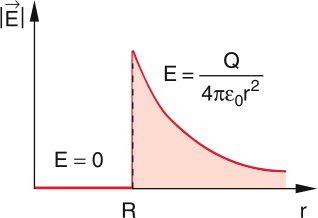
\includegraphics[width=5cm]{image/1/6.1}
    \end{minipage}
    \hspace{2cm}
    \begin{minipage}[b]{0.3\textwidth}
        \centering
        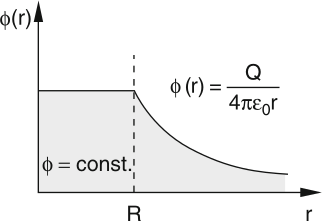
\includegraphics[width=5cm]{image/1/6.2}
    \end{minipage}
\end{figure}

\paragraph{Leiten Sie mit Hilfe des Gauß‘schen Gesetzes einen Ausdruck für das elektrische Feld und
das elektrostatische Potenziale eines homogen geladenen Kugelvolumens her. Erstellen Sie
ein Diagramm der beiden Größen als Funktion des Zentrumsabstandes.}

\begin{equation}
    \oint_{A} \bold{E} d\bold{A}
    = \frac{Q}{\epsilon_0}
    \implies
    \bold{E(r)} =
    \begin{cases}
        \frac{Q r}{4 \pi \epsilon_0 R^3} \bold{\hat{r}} ~für~ r<R \\
        \frac{Q}{4 \pi \epsilon_0 r^2} \bold{\hat{r}} ~für~ r>R
    \end{cases}
\end{equation}
\begin{equation}
    \phi(\bold{r})
    = \int_{\bold{r}}^\infty \bold{E} d\bold{s}
    = \begin{cases}
        \frac{Q}{4 \pi \epsilon_0 R} \left( \frac{3}{2} - \frac{r^2}{2 R^2} \right) ~für~ r<R \\
        \frac{Q}{4 \pi \epsilon_0 r} ~für~ r>R
    \end{cases}
\end{equation}

\begin{figure}[H]
    \centering
    \begin{minipage}[b]{0.3\textwidth}
        \centering
        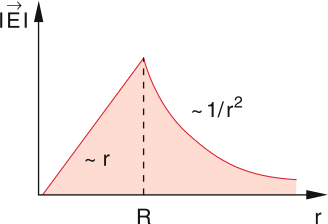
\includegraphics[width=5cm]{image/1/7.1}
    \end{minipage}
    \hspace{2cm}
    \begin{minipage}[b]{0.3\textwidth}
        \centering
        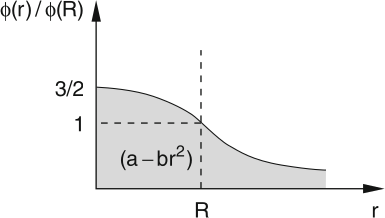
\includegraphics[width=5cm]{image/1/7.2}
    \end{minipage}
\end{figure}

\paragraph{Leiten Sie mit Hilfe des Gauß‘schen Gesetzes einen Ausdruck für das elektrische Feld und
das elektrostatische Potenziale einer homogen geladenen, sehr langen Zylinderfläche her.
Erstellen Sie ein Diagramm der beiden Größen als Funktion des Zentrumsabstandes.}

\begin{equation}
    \oint_{A} \bold{E} d\bold{A}
    = \frac{Q}{\epsilon_0}
    = \frac{\lambda l}{\epsilon_0}
    = E(r) \cdot 2 \pi r l
    \implies
    E(r) =
    \begin{cases}
        0 ~für~ r<R \\
        \frac{\lambda}{2 \pi \epsilon_0 r} ~für~ r>R
    \end{cases}
\end{equation}
\begin{equation}
    \phi(r)
    = \int_{r}^R E ds
    = \begin{cases}
        0 ~für~ r<R \\
        \frac{\lambda}{2 \pi \epsilon_0} \cdot ln \left( \frac{R}{r} \right) ~für~ r>R
    \end{cases}
\end{equation}

Als Potentialreferenz wird hierbei $R$ anstatt $\infty$ verwendet.

\begin{figure}[H]
    \centering
    \begin{minipage}[b]{0.3\textwidth}
        \centering
        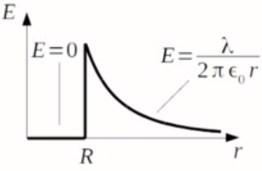
\includegraphics[height=3cm]{image/1/8.1}
    \end{minipage}
    \hspace{2cm}
    \begin{minipage}[b]{0.3\textwidth}
        \centering
        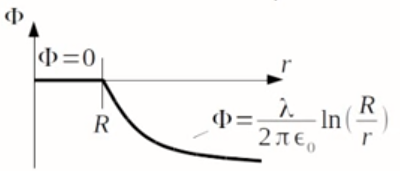
\includegraphics[height=3cm]{image/1/8.2}
    \end{minipage}
\end{figure}

\paragraph{Leiten Sie mit Hilfe des Gauß‘schen Gesetzes einen Ausdruck für das elektrische Feld und
das elektrostatische Potenziale eines homogen geladenen, sehr langen Zylindervolumnes
her. Erstellen Sie ein Diagramm der beiden Größen als Funktion des Zentrumsabstandes.}

\begin{equation}
    \oint_{A} \bold{E} d\bold{A}
    = \frac{Q}{\epsilon_0}
    = \frac{\lambda l}{\epsilon_0}
    = E(r) \cdot 2 \pi r l
    \implies
    E(r) =
    \begin{cases}
        \frac{\lambda r}{2 \pi \epsilon_0 R^2} ~für~ r<R \\
        \frac{\lambda}{2 \pi \epsilon_0 r} ~für~ r>R
    \end{cases}
\end{equation}
\begin{equation}
    \phi(r)
    = \int_{r}^R E ds
    = \begin{cases}
        \frac{\lambda}{4 \pi \epsilon_0} \cdot (1 - \frac{r^2}{R^2}) ~für~ r<R \\
        \frac{\lambda}{2 \pi \epsilon_0} \cdot ln \left( \frac{R}{r} \right) ~für~ r>R
    \end{cases}
\end{equation}

Als Potentialreferenz wird hierbei $R$ anstatt $\infty$ verwendet.

\begin{figure}[H]
    \centering
    \begin{minipage}[b]{0.3\textwidth}
        \centering
        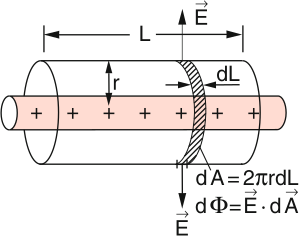
\includegraphics[width=5cm]{image/1/9.1}
    \end{minipage}
    \hspace{2cm}
    \begin{minipage}[b]{0.3\textwidth}
        \centering
        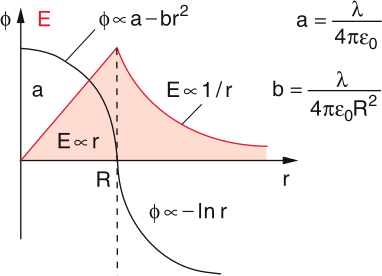
\includegraphics[width=5cm]{image/1/9.2}
    \end{minipage}
\end{figure}

\paragraph{Leiten Sie mit Hilfe des Gauß‘schen Gesetzes einen Ausdruck für das elektrische Feld und
das elektrostatische Potenzial einer homogen geladenen, unendlich großen, ebenen Fläche
her. Erstellen Sie ein Diagramm der beiden Größen als Funktion des Abstandes von der
Fläche.}

\begin{equation}
    \phi = 2 A E = \frac{Q}{\epsilon_0} = \frac{\sigma A}{\epsilon_0}
    \implies
    E = sgn(z) \cdot \frac{\sigma}{2 \epsilon_0}
\end{equation}
\begin{equation}
    \phi = \int_{z}^0 E ds = - E \cdot z = - \frac{\sigma z}{2 \epsilon_0}
\end{equation}

Als Potentialreferenz wird hierbei $0$ anstatt $\infty$ verwendet.

\begin{figure}[H]
    \centering
    \begin{minipage}[b]{0.3\textwidth}
        \centering
        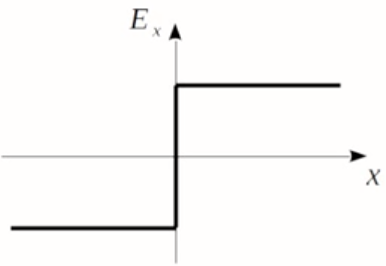
\includegraphics[width=5cm]{image/1/10.1}
    \end{minipage}
    \hspace{2cm}
    \begin{minipage}[b]{0.3\textwidth}
        \centering
        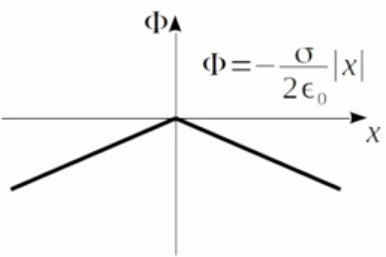
\includegraphics[width=5cm]{image/1/10.2}
    \end{minipage}
\end{figure}

\paragraph{Berechnen Sie das elektrische Feld einer Anordnung aus zwei sehr großen, parallelen,
homogen geladenen ebenen Flächen mit unterschiedlicher Flächenladungsdichte und
endlichem Abstand.}

\paragraph{Berechnen Sie das elektrische Feld einer Anordnung aus zwei homogen geladenen
Kugelflächen mit unterschiedlicher Gesamtladung. Der Abstand der Kugelmittelpunkte ist
größer als die Summe der Kugelradien.}

\paragraph{Berechnen Sie die Kraft, das Drehmoment und die potenzielle Energie eines Dipols im
homogenen elektrischen Feld.}

\begin{equation}
    \bold{F} = \bold{F_1} + \bold{F_2} = Q\bold{E} - Q\bold{E} = 0
\end{equation}
\begin{equation}
    \bold{M}
    = Q (\bold{r_1} \times \bold{E}) - Q (\bold{r_2} \times \bold{E})
    = Q \bold{d} \times \bold{E}
    = \bold{p} \times \bold{E}
\end{equation}
\begin{equation}
    W_{pot} = Q (\phi_1 - \phi_2)
\end{equation}

\begin{figure}[H]
    \centering
    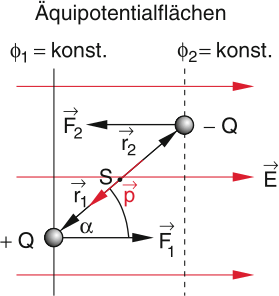
\includegraphics[width=5cm]{image/1/13}
\end{figure}

\paragraph{Berechnen Sie die Kraft auf einen Dipol in einem inhomogenen elektrischen Feld. Schreiben
Sie eine Näherung für diese Kraft für den Grenzfall eines sehr kleinen Dipols an.}

\begin{equation}
    \bold{F} = \bold{F_+} + \bold{F_-} = q [ \bold{E} (\bold{r_-} + d) - \bold{E(r_-)}]
\end{equation}
\begin{equation}
    \bold{F} \approx Q \bold{d} \frac{d\bold{E(r)}}{d\bold{r}} = \bold{p} \times \nabla \bold{E(r)}
\end{equation}

\begin{figure}[H]
    \centering
    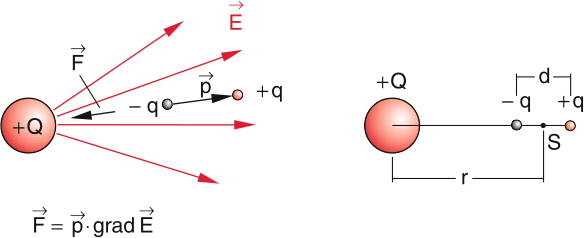
\includegraphics[width=8cm]{image/1/14}
\end{figure}

\newpage

\section{Materie im elektrischen Feld}

\paragraph{Was ist ein elektrischer Leiter und was passiert wenn ein elektrischer Leiter in ein
statisches elektrisches Feld gebracht wird. Wie nennt man den Effekt und welche Bedingungen muss das
elektrische Feld und -Potenzial an der Leiteroberfläche und innerhalb des Leiters erfüllen?} ~

Ein elektrischer Leiter ist ein Medium, welches eine hohe Dichte frei beweglicher Ladungsträger und
daher eine gute elektrische Leitfähigkeit sowie einen möglichst geringen elektrischen Widerstand
besitzt. Er ist dadurch zum Transport geladener Teilchen geeignet, welchen man auch als elektrischen
Strom nennt.

Es kommt zu einer Ladungsverschiebung aufgrund des E-Feldes, wodurch sich ein Gegenfeld aufbaut und
das äußere Feld kompensiert. Das Innere des Leiters wird dadurch feldfrei, man spricht von Influenz.
Die beweglichen Ladungsträger befinden sich an der Leiteroberfläche und bilden somit eine
Äquipotentialfläche, auf welche die Feldlinien senkrecht stehen. Das Potential im Inneren des
Leiters ist konstant.

\paragraph{Was ist ein Kondensator? Warum kann man eindeutig eine elektrische Spannung zwischen zwei
entgegengesetzt geladenen Metallkörpern angeben? Wie ist die elektrische Kapazität definiert und
wovon hängt deren Größe ab?} ~

Ein Kondensator ist ein elektrisches Bauelement mit der Fähigkeit, elektrische Ladung und die damit
zusammenhängende Energie in einem elektrischen Feld zu speichern.

Da das elektrische Feld im Raum zwischen den Leiterflächen proportional zur Ladung $Q$ und die
Spannung $U$ wegen $U = \int \bold{E} d\bold{s}$ proportional zu $Q$ ist gilt die Beziehung
\begin{equation}
    C = \frac{Q}{U} \text{ ,}
\end{equation}
wobei die in Farad angegebene Proportionalitätskonstante $C$ die Kapazität des Kondensators ist.
Diese ist sowohl von der Geometrie als auch vom verwendeten Dielektrikum zwischen den Leitern
abhängig.

\paragraph{Ein Plattenkondensator mit der Kapazität $C$ und Plattenabstand $d_C$ ist auf die Spannung
$U$ geladen und von der Spannungsquelle getrennt. Nun wird eine isolierte Metallplatte (Dicke
$d_M<d_C$) parallel zu den Kondensatorplatten zwischen diese eingeschoben. Beschreiben Sie was
passiert. Berechnen Sie die elektrische Feldstärken vor- und nach Einschieben der Platte. Zeichnen
Sie ein Diagramm der elektrischen Feldstärke und des elektrischen Potenzials zwischen den
Kondensatorplatten vor und nach Einschieben der Metallplatte.} ~

Aufgrund der Influenz erfolgt eine Ladungsverschiebung in der Platte, auf dessen Oberfläche sich nun
die Ladungsträger sammeln und ein Gegenfeld bewirken, welches das Innere der Platte feldfrei macht.
Dadurch sinkt auch die Spannung, da effektiv weniger Plattenabstand vorhanden ist - die Kapazität
$C$ des Kondensators steigt.

\begin{equation}
    \text{vorher:} ~~~
    E_V = \frac{Q}{A \cdot \epsilon_0} = \frac{U}{d_C}
\end{equation}
\begin{equation}
    \text{nachher:} ~~~
    E_V = \frac{U}{d_C - d_M} ~~~
    E_M = 0
\end{equation}

\begin{figure}[H]
    \centering
    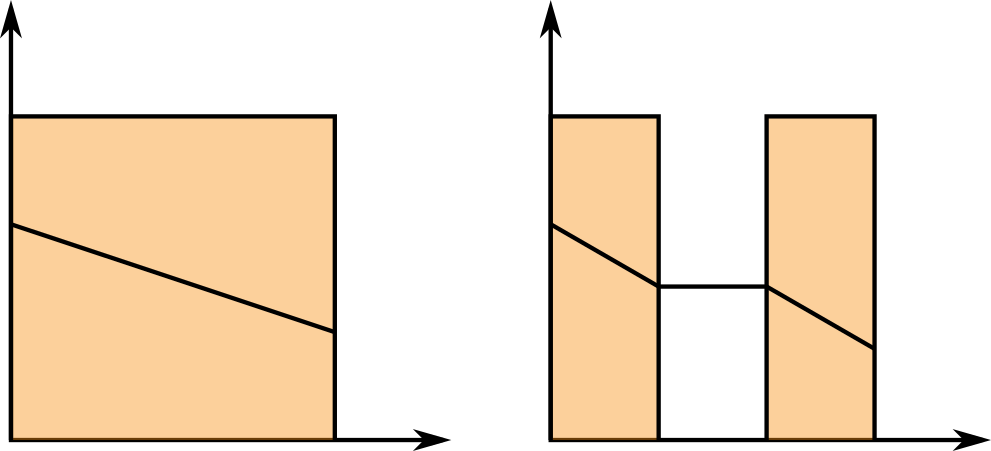
\includegraphics[width=5cm]{image/2/3}
\end{figure}

\paragraph{Ein Plattenkondensator mit der Kapazität $C$ und Plattenabstand $d_C$ ist an eine
Spannungsquelle mit der Spannung $U$ angeschlossen. Nun wird eine dielektrische Platte (Dicke $d_D$,
Permitivität $\epsilon_D$) parallel zu den Kondensatorplatten zwischen diese eingeschoben.
Beschreiben Sie was passiert. Berechnen Sie die elektrische Feldstärken und die elktrischen
Verschiebungsdichten vor- und nach einschieben der Platte. Zeichnen Sie ein Diagramm der
elektrischen Feldstärke, der dielektrischen Verschiebungsdichte und des elektrischen Potenzials
zwischen den Kondensatorplatten vor und nach Einschieben der dielektrischen Platte.} ~

Durch das Feld des Kondensators werden die festen Moleküle im Dielektrikum polarisiert - es bildet
sich ein Gegenfeld, welches das äußere jedoch nicht vollständig kompensiert. Die Feldstärke und die
Spannung sinken um den Faktor $\epsilon_D$, die Kapazität steigt entsprechend um den Faktor
$\epsilon_D$.

\begin{equation}
    \text{vorher:} ~~~
    E_V = \frac{Q}{A \cdot \epsilon_0} = \frac{U}{d_C} ~~~
    D_V = E_V \cdot \epsilon_0
\end{equation}
\begin{equation}
    \text{nachher:} ~~~
    E_V = \frac{U}{d_C - d_D + \frac{d_D}{\epsilon_D}} ~~~
    E_D = \frac{E_V}{\epsilon_0} ~~~
    D_V = D_D
\end{equation}

\begin{figure}[H]
    \centering
    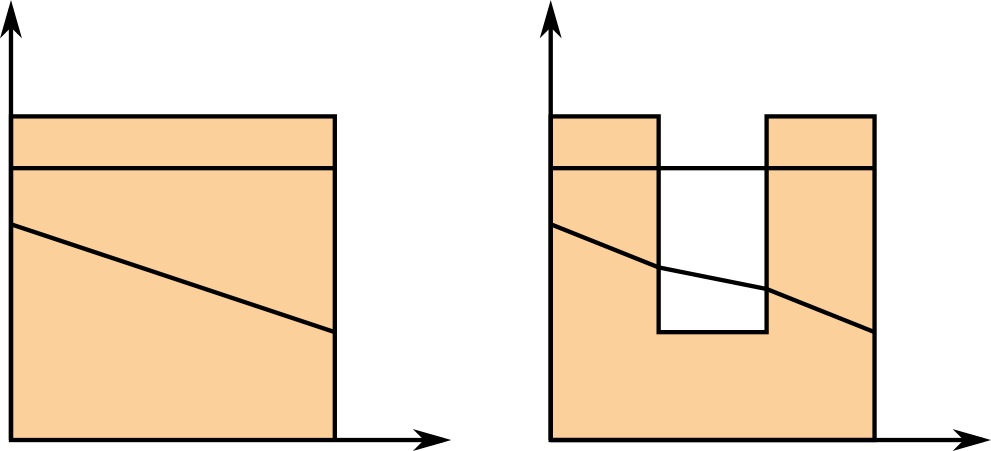
\includegraphics[width=5cm]{image/2/4}
\end{figure}

\paragraph{Ein Plattenkondensator mit Fläche $A$, Plattenabstand $d$, gefüllt mit einem Dielektrikum
mit der relativen Permittivität $\epsilon$ ist mit der Ladung $Q$ geladen. Wie groß ist die in ihm
gespeicherte Energie?}

\begin{equation}
    E_{el} = \frac{Q^2}{2 \cdot C} = \frac{Q^2}{2 \cdot \epsilon \epsilon_0 \frac{A}{d}}
\end{equation}

\paragraph{Was ist der Unterschied zwischen Polarisation und Influenz? Welche Arten von Polarisation
können bei einem Dielektrikum auftreten? Was für Voraussetzungen müssen die Moleküle des
Dielektrikums dafür erfüllen?} ~

Unter Influenz versteht man die räumliche Verschiebung frei beweglicher Ladungsträger im Leiter
durch ein äußeres Feld, wodurch sich ein (meist das äußere Feld kompensierendes) Gegenfeld bildet.
Die Polarisation ist ein vergleichbarer Effekt im Dielektrikum, allerdings können hier die Ladungen
nur innerhalb der Atome oder Moleküle verschoben werden. Es entsteht ein schwächeres Gegenfeld als
im Leiter, das äußere Feld kann nicht kompensiert werden.

\begin{itemize}
    \item Induzierte Polarisation: Die Polarisierbarkeit (Verschiebbarkeit der negativen und
    positiven Ladungsträger im Atom oder Molekül relativ zueinander) muss ausreichend groß sein.
    
    \item Orientierungspolarisation: Die Schwerpunkte der positiven und negativen Ladungen müssen
    deutlich voneinander getrennt sein, man spricht von Dipolmolekülen oder permanenten Molekülen.
    Ein Beispiel hierfür sind Wassermoleküle.
\end{itemize}

\paragraph{Beschreiben Sie die Größen elektrische Polarisation, Suzeptibilität,
Dielektrizitätskonstante, dielektrische Verschiebungsdichte und elektrische Feldstärke. Wie hängen
sie zusammen und welche Einheiten haben sie?}

\begin{itemize}
    \item Polarisation $\bold{P}$: Beschreibt, wie stark ein Dielektrikum polarisiert ist
    beziehungsweise kennzeichnet die Stärke des Dipolmoments in dielektrischen Material.
    $[P] = \si{\A\s\per\m^2}$
    
    \item Suszeptibilität (Reizbarkeit) $\chi$: Materialeigenschaft, welche die Fähigkeit zur
    elektrischen Polarisierung in einem eingeprägten elektrischen Feld angibt. $[\chi] = 1$
    
    \begin{equation}
        \chi = \frac{P}{E \cdot \epsilon_0}
    \end{equation}
    
    \item Dielektrizitätskonstante $\epsilon$: Gibt die Polarisationsfähigkeit eines Materials
    durch elektrische Felder an. $[\epsilon] = \si{\A\s\per\V\per\m}$
    
    \item Dielektrische Verschiebungsdichte $\bold{D}$: Ist ein Maß für die auf einer Fläche im
    elektrischen Feld durch Influenz hervorgerufenen Ladung. $[D] = \si{\coulomb\per\m^2}$
    
    \begin{equation}
        \bold{D} = \epsilon \epsilon_0 \bold{E} = \epsilon_0 \bold{E} + \bold{P}
    \end{equation}
    
    \item Elektrische Feldstärke $\bold{E}$: Beschreibt die Stärke und Richtung eines elektrischen
    Feldes, also die Fähigkeit des Feldes, Kraft auf Ladungen auszuüben. $[E] = \si{\V\per\m}$
\end{itemize}

\paragraph{Schreiben Sie die Feldgleichungen der Elektrostatik in Materie an (Integralform) und
benennen Sie alle vorkommenden Größen inklusive Einheiten.}

\begin{equation}
    \oint_A \bold{E} d\bold{A} = \frac{Q}{\epsilon_0} ~~~ \oint \bold{E} d\bold{s} = 0
\end{equation}

\begin{itemize}
    \item $A$: Oberfläche des Volumens $[A] = \si{\m^2}$
    \item $\bold{E}$: Elektrische Feldstärke $[E] = \si{\V\per\m}$
    \item $Q$: Eingeschlossene Ladung $[Q] = \si{\coulomb}$
    \item $\epsilon_0$: Elektrische Feldkonstante $[\epsilon_0] = \si{\A\s\per\V\per\m}$
\end{itemize}

\paragraph{Ein Elektron bewegt sich zum Zeitpunkt $t_0$ mit der Geschwindigkeit $v_0$ senkrecht zu
den elektrischen Feldlinien in einem elektrischen Feld. Stellen Sie die Bewegungsgleichung auf und
beschreiben Sie die weitere Bahn des Elektrons.}

\begin{equation}
    F = q \cdot E = m \cdot a_y
    \implies
    a_y = \frac{E \cdot e}{m}
\end{equation}
\begin{equation}
    s_x(t) = v_0 \cdot t
\end{equation}
\begin{equation}
    s_y(t) = \frac{1}{2} \cdot a_y \cdot t^2
\end{equation}

Außerhalb des Feldes gilt für die Beschleunigung $a_y = 0$, die weitere Kurve entspricht einer
Geraden.

\paragraph{Beschreiben Sie Zweck und Funktionsprinzip des Millikan Versuches. Wie kann die Masse und
die elektrostatische Kraft auf die Öltröpfchen bestimmt werden und wie bestimmt man deren Ladung?} ~

Der Millikan-Versuch dient der experimentellen Ermittlung der Elementarladung $e$. Durch Zerstäuben
von Öl werden kleine Öltröpfchen erzeugt, welche aufgrund der Reibung beim Zerstäubungsvorgang die
Ladung $n \cdot e$ besitzen und zwischen die horizontalen Platten eines Kondensators diffundieren.

Im feldfreien Kondensator wird die Schwerkraft $m \cdot g$ durch die Summe der Auftriebskraft
$F_A = \rho_{Luft} \cdot \frac{4}{3} \pi R^3 \cdot g$ und der Reibungskraft
$F_R = 6 \pi \eta R \cdot v$ kompensiert. Die sich einstellende konstante Sinkgeschwindigkeit kann
gemessen werden, wodurch sich der Radius und in weiterer Folge die Masse des Tröpfchens ergibt.

Durch Anlegen einer geeigneten Spannung am Kondensator kann nun das Tröpfchen im E-Feld in Schwebe
gehalten werden. Eine Ladungsänderung des Tröpfchens durch beispielsweise Röntgenstrahlung erfordert
eine Spannungsänderung, um den Schwebezustand aufrecht zu erhalten. Mithilfe der bekannten
Spannungswerte kann nun $n$ und in weiterer Folge $e$ bestimmt werden.

\begin{figure}[H]
    \centering
    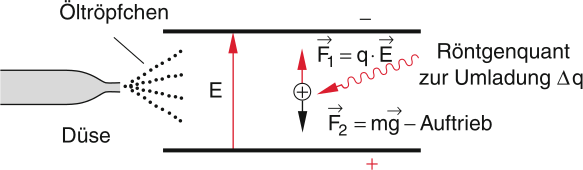
\includegraphics[width=10cm]{image/2/10}
\end{figure}

\newpage

\section{Elektrischer Strom I}

\paragraph{Was bedeuten die Begriffe elektrischer Strom, Stromdichte und Driftgeschwindigkeit und
wie sind sie miteinander verknüpft? Welche Einheiten habe diese Größen? Sind es skalare oder
vektorielle Grössen?} ~

\begin{itemize}
    \item Elektrischer Strom $I$: Transport von elektrischen Ladungsträgern $[I] = \si{\A}$
        \begin{equation}
            I = \int_A \bold{j} d\bold{A}
        \end{equation}
    
    \item Stromdichte $\bold{j}$: Verhältnis der Stromstärke $I$ zur Verfügung stehenden
        Querschnittsfläche $A$ $[j] = \si{\A\per\m^2}$
        \begin{equation}
            \bold{j} = n \cdot q \cdot \bold{v_D} 
        \end{equation}
    
    \item Driftgeschwindigkeit $\bold{v_D}$: Die mittlere Geschwindigkeit der Ladungsträger aufgrund
        eines äußeren Feldes $[v] = \si{\m\per\s}$
\end{itemize}

\paragraph{Was bedeuten die Begriffe Beweglichkeit und elektrische Leitfähigkeit und spezifischer
Widerstand? Welche Einheit haben sie und in welcher Beziehung stehen sie zur Stromdichte?} ~

\begin{itemize}
    \item Beweglichkeit $\mu$: Gibt die Driftgeschwindigkeit der Ladungsträger bei einer
        elektrischen Feldstärke von \SI{1}{\V\per\m} an $[\mu] = \si{\m\squared\per\V\per\s}$
        \begin{equation}
            \bold{j} = \sigma \cdot \frac{\bold{v_d}}{\mu}
        \end{equation}
    
    \item Elektrische Leitfähigkeit $\sigma$: Fähigkeit eines Stoffes, den elektrischen Strom zu
        leiten $[\sigma] = \si{\A\per\V\per\m}$
        \begin{equation}
            \bold{j} = \sigma \cdot \bold{E}
        \end{equation}
    
    \item Spezifischer Widerstand $\rho_s$: Kehrwert der elektrischen Leitfähigkeit
        $[\rho_s] = \si{\ohm\m}$
        \begin{equation}
            \bold{E} = \rho \cdot \bold{j}
        \end{equation}
\end{itemize}

\paragraph{Was besagt das Ohm‘sche Gesetz? Schreiben Sie das Ohm‘sche Gesetz in seiner lokalen und
integralen Form an. Was ist ein Ohm‘scher Leiter?} ~

Die Stärke des durch ein Objekt fließenden elektrischen Stroms ist proportional der elektrischen
Spannung.
\begin{equation}
    \bold{j} = \sigma \cdot \bold{E} ~~~ R = \int_0^l \frac{\rho}{s} dl
\end{equation}
Einen Leiter, für welchen $\rho_s$ unabhängig von Strom $I$ und Spannung $U$ sind, nennt man
ohm'schen Leiter. Die Spannung $U$ und der Strom $I$ sind also über $R$ proportional zueinander.

\paragraph{Eine ideale Spannungsquelle liefert eine Klemmspannung von \SI{10}{\V}. Entwerfen und
dimensionieren Sie eine einfache Schaltung aus Widerständen, die es ihnen erlaubt eine Spannung von
\SI{4}{\V} abzugreifen. Der gesamtwiderstand der Schaltung sollte \SI{10}{\kilo\ohm} sein.}

\begin{equation}
    I = \frac{U_0}{R_{ges}} = \frac{U_1}{R_1} = \frac{U_2}{R_2}
\end{equation}
\begin{equation}
    \begin{rcases}
        R_1 = R_{ges} \cdot \frac{U_1}{U_0} \\
        R_2 = R_1 \cdot \frac{U_2}{U_1}
    \end{rcases}
    \implies
    R_2 = R_{ges} \cdot \frac{U_2}{U_0} = \SI{4}{\kilo\ohm}
\end{equation}
\begin{equation}
    R_1 = R_{ges} - R_1 = \SI{6}{\kilo\ohm}
\end{equation}

\begin{figure}[H]
    \centering
    \includegraphics[width=5cm]{image/3/4}
\end{figure}

\paragraph{Das Material eines metallischen Leiters (Draht) mit konstanter Querschnittsfläche $F$ und
einer Länge $L$, habe den spezifischen Widerstand $\rho$. Berechnen Sie den Ohm‘schen Widerstand des
Drahtes.} ~
\begin{equation}
    R = \rho \cdot \frac{L}{F}
\end{equation}

\paragraph{Beschreiben Sie den Ladungsvorgang eines Kondensators, der über einen Widerstand
plötzlich mit einer idealen Spannungsquelle verbunden wird (Strom und Spannungen als Funktion der
Zeit).} ~

\begin{equation}
    U(t) = U_0 \cdot \left( 1 - e^{-t /(R C)} \right)
\end{equation}
\begin{equation}
    I(t) = I_0 \cdot e^{-t /(R C)}
\end{equation}

\begin{figure}[H]
    \centering
    \begin{minipage}[b]{0.3\textwidth}
        \centering
        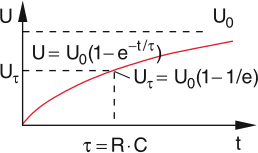
\includegraphics[width=5cm]{image/3/6.1}
    \end{minipage}
    \hspace{2cm}
    \begin{minipage}[b]{0.3\textwidth}
        \centering
        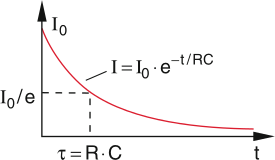
\includegraphics[width=5cm]{image/3/6.2}
    \end{minipage}
\end{figure}

\paragraph{Beschreiben Sie den Entladungsvorgang eines geladenen Kondensators, dessen Kontakte über
einen Widerstand plötzlich verbunden werden (Strom und Spannungen als Funktion der Zeit).} ~

\begin{equation}
    U(t) = U_0 \cdot e^{-t /(R C)}
\end{equation}
\begin{equation}
    I(t) = I_0 \cdot e^{-t /(R C)}
\end{equation}

\begin{figure}[H]
    \centering
    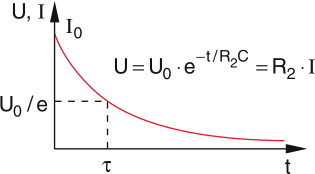
\includegraphics[width=5cm]{image/3/7}
\end{figure}

\paragraph{Beschreiben Sie die elektrische Leitung in Metallen. Wie ändert sich der spezifische
Widerstand mit der Temperatur? Begründen Sie.} ~

Das Anlegen einer Spannung bewirkt ein elektrisches Feld im Metall, welches die Elektronen zum
positiven Pol der Spannungsquelle hin beschleunigt. Duch die Kollision der Elektronen mit den Ionen
im Kristallgitter verlieren erstere kinetische Energie, welche in Wärmeenergie umgewandelt wird.

Bei höheren Temperaturen kommt es zu stärkeren Schwingungen der Metallionen, wodurch die Bewegung
der Elektronen noch stärker beschränkt wird. Der spezifische Widerstand steigt also mit der
Temperatur.

Bei sehr tiefen Temperaturen können viele Metalle ihren Widerstand völlig verlieren, man spricht
dann von Supraleitung.

\paragraph{Beschreiben Sie die elektrische Leitung in Halbleitern. Wie ändert sich der spezifische
Widerstand mit der Temperatur? Begründen Sie.} ~

Die Atome im Halbleiter bilden stabile Elektronenpaarbindungen, bei tiefen Temperaturen sind also
keine freien Elektronen verfügbar. Mit steigender Temperatur können aufgrund ihres höheren
Energie-Niveaus jedoch Elektronen frei werden, die Leitfähigkeit steigt also währen der elektrische
Widerstand mit steigender Temperatur sinkt.

Durch das Fehlen von Elektronen im Gitter entstehen Löcher, welche als positive Ladungsträger
betrachtet werden können. Diese Löcher werden durch von Loch zu Loch springende Elektronen gefüllt,
wodurch sie scheinbar in entgegengesetzter Richtung der Elektronen wandern und damit ebenso dem
Ladungstransport dienen.

\paragraph{Beschreiben Sie die elektrische Leitung in Gasen.} ~

Der Ladungstransport in ionisierten Gasen, die auch als Plasma bezeichnet werden, erfolgt sowohl
durch Elektronen als auch durch Ionen. Neben der Existenz dieser frei beweglichen Ladungsträger ist
ein elektrisches Feld Voraussetzung für die Leitung in Gasen.

Die Erzeugung von Ladungsträgern im Gas kann über verschiedene Methoden erfolgen:

\begin{itemize}
    \item Thermische Ionisation: Durch eine Kombination der thermischen Anregung und der damit
        initiierten chemischen Prozesse entstehen Ladungsträger. Die erforderliche, sehr hohe
        Temperatur kann durch Verwendung eines Katalysators verringert werden.
    
    \item Elektronenstoßionisation: Elektronen mit ausreichend hoher Energie können beim Stoß mit
        Atomen oder Molekülen Elektronen aus der Elektronenhülle herausschlagen und damit ein
        Elektron-Ion-Paar bilden.
    
    \item Photoionisation: Durch kurzwellige Strahlung wie etwa UV- oder Röntgenstrahlung können
        Atome oder Moleküle aufgrund der hochenergetischen Photonen ihrer Elektronen beraubt werden.
        Dies führt ebenfalls zur Entstehung von Elektron-Ion-Paaren.
\end{itemize}

\paragraph{Beschreiben Sie die Ionenleitung in Flüssigkeiten.} ~

Flüssigkeiten, in denen Säuren, Laugen oder Salze gelöst sind, nennt man Elektrolyte. Im Gegensatz
zu Metallen ist hier der Stromdurchgang mit einer chemischen Zersetzung des Elektrolyten verbunden.
Sowohl an der Anode als auch an der Kathode werden Stoffe in fester oder gasförmiger Form
abgeschieden.

Durch Dissoziation - also durch Aufspaltung von Molekülen in kleinere Bestandteile - entstehen
positiv und negativ geladene Ionen. Diese ermöglichen bei einer angelegten Spannung den
Ladungstransport mit der sogenannten Driftgeschwindigkeit. Während die positiven Ionen zur Kathode
wandern und dort Elektronen aufnehmen geben die negativen Ionen an der Anode ihre überschüssigen
Elektronen ab. Dabei scheiden sie als neutrale Atome an der jeweiligen Elektrode ab.

\begin{figure}[H]
    \centering
    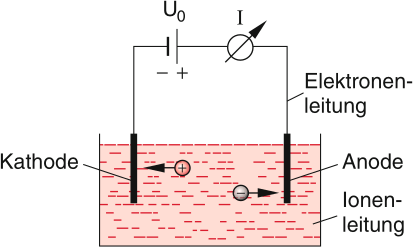
\includegraphics[width=7cm]{image/3/11}
\end{figure}

\newpage

\section{Elektrischer Strom II}

\paragraph{Beschreiben Sie die Funktionsweise eines galvanischen Elementes. Wodurch ist die
erzielbare Spannung bestimmt?}

\paragraph{Beschreiben Sie die Funktionsweise einer Brennstoffzelle.}

\paragraph{Beschreiben Sie den Seebeck-Effekt und die Ursache der Thermospannung.}

\paragraph{Was ist der Innenwiderstand einer Spannungsquelle? Wie groß ist der Innenwiderstand einer
idealen Spannungsquelle bzw. einer idealen Stromquelle?}

\paragraph{Wie kann man den Kurzschlussstrom und den Innenwiderstand eines Akkumulators durch
Strom und Spannungsmessung ermitteln, ohne den Akku wirklich kurz zu schließen? Der Akkumulator sei
in guter Näherung eine lineare Spannungsquelle. Schaltungsskizze!}

\paragraph{Zeichnen Sie das Ersatzschaltbild einer mit einem Widerstand $R$ belasteten linearen
Spannungsquelle mit Innenwiderstand $R_i$ und elektromotorischer Kraft $U$. Berechnen Sie einen
Ausdruck für die Klemmspannnung.}

\paragraph{Was versteht man unter Leistungsanpassung bei einer Spannungsquelle? Bei welchem Last-
bzw. Innenwiderstand ist dies erfüllt?}

\paragraph{Beschreiben und erklären Sie die Funktionsweise eines Dual-Slope Analog-Digital
Umsetzers.}

\paragraph{Beschreiben und erklären Sie die Funktionsweise eines Flash Analog-Digital Umsetzers.}

\paragraph{Aus welchen Beiträgen setzt sich die Gesamtunsicherheit eines Digitalvoltmeters
zusammen?}

\paragraph{Die maximal messbare Spannung eines Voltmeters mit Innenwiderstand $R_i$ ist $U_m$. Der
Messbereich soll auf $10 \cdot U_m$ erweitert werden. Zeichnen und dimensionieren Sie eine
Widerstandsschaltung die dies ermöglicht. Wie groß ist der Gesamtwiderstand dieser Schaltung?}

\paragraph{Die maximal mit einem Amperemeter (Innenwiderstand $R_i$) messbare Strom sei $I_m$. Der
Messbereich soll auf $10 \cdot I_m$ erweitert werden. Zeichnen und dimensionieren Sie eine
Widerstandsschaltung die dies ermöglicht. Wie groß ist der Gesamtwiderstand dieser Schaltung?}

\newpage

\section{Statische Magnetfelder}

\paragraph{Schreiben Sie das Ampere‘sche Gesetz an. Leiten Sie daraus einen Ausdruck für das
Magnetfeld eines geraden, sehr langen, zylindrischen Leiters ab, durch den ein elektrischer Strom
mit über den Leiterquerschnitt homogener Stromdichte fließt.}
Das Ringintegral entlang einer geschlossenen Magnetfeldlinie, ist immer gleich dem eingeschlossenen Strom mal der magnetischen Feldkonstante,
wie aus dem Amperschen Gesetz \ref{AmperschesGesetz} ersichtlicht wird.  
\begin{equation}
    \oint \textbf{B} \hspace{0.2em} d\textbf{s} = \mu_0\cdot I
\end{equation}
Wählt man nun als Integrationsweg die den Draht umschließende Feldlinie mit dem Abstand $r$, so ergibt sich:
\begin{equation}
    \int_{0}^{2\pi} rBd\phi = 2 \pi r B(r) = \mu_0\cdot I
\end{equation}
\begin{equation}
    B(r) = \frac{\mu_0\cdot I}{2 \pi r} \hspace{2.5em} \text{für} \hspace{1em} r > r_0
\end{equation}
\begin{equation}
    B(r) = \frac{\mu_0\cdot I}{r_{0}^{2} 2 \pi} \cdot r  \hspace{2.5em} \text{für} \hspace{1em} r < r_0
\end{equation}
\paragraph{Schreiben Sie das Ampere‘sche Gesetz an. Leiten Sie daraus einen Ausdruck für das
Magnetfeld im Inneren einer geraden, sehr langen, zylindrischen Leiterspule ab.}
Der Integrationsweg wird so gewählt, dass nur der Teil im Inneren der Spule einen Beitrag leistet.
\begin{figure}
    \label{Integrationsweg}
    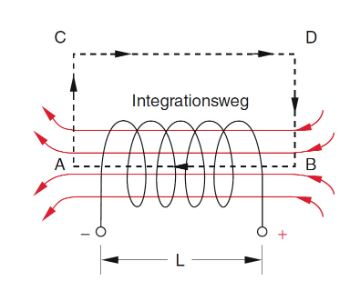
\includegraphics[height=5cm]{image/5/5.2.JPG}
\end{figure}
$N$ ist in diesem Zusammenhang die Anzahl der Windungen.
\begin{equation}
    \int_A^{B} B \hspace{0.2em} ds = B\cdot L = N\mu_0 I
\end{equation}
\begin{equation}
    B = \frac{N}{L}\mu_0 I \hspace{5em} \text{mit} \hspace{1em} \frac{N}{L} = n \hspace{0.5em} \text{(Windungsdichte)}
\end{equation}
\paragraph{Schreiben Sie einen Ausdruck für die Lorentzkraft (nicht die verallgemeinerte
Lorentzkraft) einer bewegten Ladung im Magnetfeld an. Beschreiben Sie alle verwendeten Formelsymbole
und leiten Sie damit die Kraft auf einen geraden, stromdruchflossenen Leiter im homogenen Magnetfeld
her.}
\begin{equation}
    F = q(textbf{v} \times \textbf{B})
\end{equation}
\begin{itemize}
    \item $q$ Ladung auf die die Kraft wirkt 
    \item \textbf{v} die Geschwindigkeit des Ladungsträgers
    \item \textbf{B} Magnetfeld, welches der Ladungsträgert passiert
\end{itemize}
\begin{equation}
    d\textbf{F} = (\textbf{j} \times \textbf{B})\hspace{0.2em} dV \hspace{3em} dV = A\cdot dL \hspace{1em}\& \hspace{1em} j \cdot A = I
\end{equation}
\begin{align}
    d\textbf{F} &= I (d\textbf{L} \times \textbf{B})  \\
    \notag \\ 
    \textbf{F} &= I (\textbf{L} \times \textbf{B})
\end{align}
\paragraph{Schreiben Sie eine Ausdruck für das Magnetfeld zweier paralleler, stromdurchflossener,
zylindrischer Leiter an. Erstellen Sie ein Diagramm der magnetischen Feldstärke als Funktion des
Ortes entlang einer Linie, die die Achsen beider Leiter unter \SI{90}{\degree} schneidet. Welche
Richtung hat das Magnetfeld entlang dieser Linie?}
Das Magnetfeld des einen Leiters übt eine Kraft, abhängig von der Stromrichtung, auf den anderen aus.
Dieses Magnetfeld  $B = \frac{\mu_0 I}{2 \pi r} \cdot \hat{e}^{\phi}$ steht tangential auf konzentrischen Feldlinien.
Setzt man diesen Zusammenhang in die hergeleitete Formel der letzten Frage, so bemerkt man das $B$ orthognal auf $L$ steht. 
Somit ergibt sich:
\begin{align}
    F_1 &= I_1(L_1 \cdot \frac{\mu_0 I_2}{2 \pi r} ) \\
    \\
    \frac{F_1}{L_1} &= \frac{\mu_0}{2 \pi r} \cdot I_2 \cdot I_1
\end{align}
\paragraph{Leiten Sie ausgehend von der Kraft auf einen stromdurchflossenen, geraden Draht im
homogenen Magnetfeld einen Ausdruck für das Drehmoment einer rechteckigen Leiterschleife im
homogenen Magnetfeld her. Die Drehachse ist parallel zu zwei Seiten der Leiterschleife und senkrecht
zur Richtung des Magnetfeldes. Bei welchem Winkel zwischen Leiterschleife und Magnetfeldrichtung ist
das Drehmoment maximal? Bei welchem Winkel ist der magnetische Fluss durch die Leiterschleife
maximal?}
\begin{figure}
    label{Drehmomen}
\end{figure}

\paragraph{Ein geladenes Teilchen ist bei $t=0$ am Ort $x=(0,0,0)$ mit der Geschwindigkeit
$v=(v_x,0,v_z)$ in einem homogenen Magnetfeld $B=(0,0,B_z)$. Wie wird die weitere Bahn des Teilchens
qualitativ aussehen und warum? Berechnen Sie die Kreisfrequenz und Radius.}

\paragraph{Beschreiben Sie die Funktion und Aufbau eines Wien-Filters und leiten Sie einen Ausdruck
für die Filter-Geschwindigkeit her.}

\paragraph{Beschreiben Sie den Hall-Effekt und leiten Sie ausgehend von der Lorentzkraft einen
Ausdruck für die Hall-Spannung für einen Leiter mit rechteckigem Querschnitt im homogenen Magnetfeld
her.}

\paragraph{Wie beeinflussen Stromdichte, Querschnittsabmessungen, Ladungsträgerdichte und Ladung
der Ladungsträger die Hall-Spannung? Geben Sie an, ob die Parameter groß oder klein sein sollten, um
eine möglichst große Hall-Spannung zu beobachten.}

\newpage

\section{Materie im elektrischen Feld}

\paragraph{Ein kleiner Probekörper mit bekanntem Volumen befindet sich in einem inhomogenen
magnetischen Feld. Der Probekörper wird durch das äußere Magnetfeld magnetisiert und erfährt daher
eine Kraft. Wie groß ist diese Kraft und welche Richtung hat sie bei positiver oder negativer
magnetischer Suzeptiblität?}

\paragraph{Welche magnetischen Stoffklassen gibt es und wie unterscheiden sie sich in ihren
magnetischen Eigenschaften?}

\paragraph{Was versteht man unter Diamagnetismus und Paramagnetismus? Welche spezielle Eigenschaft
haben Moleküle oder Atome eines dia- oder paramegnetischen Stoffes?}

\paragraph{Beschreiben Sie die Eigenschaften eines ferromagnetischen Stoffes? Nennen Sie drei
Beispiele für ferromagnetische Stoffe.}

\paragraph{Was sind antiferromagnetische und ferrimagnetische Stoffe?}

\paragraph{Schreiben Sie die Feldgleichungen der Elektro- und Magnetostatik an. Welche
Stetigkeitsbedingungen müssen die elektrischen und magnetischen Felder an Grenzflächen erfüllen?}

\newpage

\section{Zeitlich veränderliche Felder}

\paragraph{Schreiben Sie das Faradaysche Induktionsgesetz an. Welche Prozesse können zu einer
induzierten Spannung in einer Leiterschleife führen?}

\paragraph{Eine quadratische Leiterschleife (Schleifenfläche A) dreht sich im homogenen Magnetfeld
mit der Winkelgeschwindigkeit $\omega$ um eine Achse, die senkrecht zu den magnetischen Feldlininen
steht. Schreiben Sie einen Ausdruck für die induzierte Spannung als Funktion des Winkels und der
Zeit an. Bei welcher Orientierung der Leiterschleife relativ zum Magnetfeld ist die induzierte
Spannung maximal (Skizze!)?}

\paragraph{Eine offene Leiterschleife befindet sich in einem homogenen Magnetfeld. Der
Flächennormalvektor steht parallel zu den Feldlinien. Die magnetische Feldstärke nimmt mit der Zeit
zu. Skizzieren Sie die Situation und zeichnen Sie die Richtung der induzierten elektrischen
Feldstärke sowie die Polarität der beiden offenen Enden der Leiterschleife ein.}

\paragraph{Beschreiben Sie Aufbau und Funktion einer Induktionsschleuder.}

\paragraph{Was versteht man unter Selbstinduktion? Was bedeutet der Selbstinduktionskoeffizient?}

\paragraph{Eine Doppelleitung besteht aus zwei zylindrischen, parallelen Leitern, durch die der
gleiche Strom aber mit unterschiedlichen Vorzeichen fließt. Fertigen Sie eine Skizze an, skizzieren
Sie das Magnetfeld der Anordnung und schreiben Sie das Magnetfeld zwischen den Leitern analytisch
an. Zeigen Sie, wie man daraus (im Prinzip) den Selbstinduktionskoeffizienten der Doppelleitung
berechnen kann.}

\paragraph{Was versteht man unter Gegeninduktion? Wie kann man sie formal beschreiben?}

\paragraph{Beschreiben Sie den Strom- und Spannungsverlauf einer Serienschaltung aus idealer
Induktivität und ohm‘schen Widerstand, wenn diese über einen Schalter mit einer idealen
Spannungsquelle verbunden werden (Einschaltvorgang). Schreiben Sie die Funktionen $I(t)$ sowie
$U(t)$ für Widerstand und Spule an und erstellen Sie die entsprechenden Diagramme.}

\paragraph{Beschreiben Sie den Strom- und Spannungsverlauf einer Serienschaltung aus idealer
Induktivität und ohm‘schen Widerstand, wenn diese über einen Schalter von einer
Spannungsquelle plötzlich getrennt werden (Ausschaltvorgang). Schreiben Sie die
Funktionen $I(t)$ sowie $U(t)$ für Widerstand und Spule an und erstellen Sie die entsprechenden
Diagramme.}

\paragraph{Wie kann man im Prinzip die Induktivität z.B. einer Spule durch eine Zeitmessung
bestimmen (Schaltplan und Beschreibung)?}

\paragraph{Zwei dünne, lange Spulen sind auf den gleichen Kern gewickelt, sodass der gesamte
magnetische Fluss der einen Spule durch die andere fließt. Berechnen Sie die in einer Spule
induzierte Spannung, wenn sich in der andern der Strom ändert. Die Spulenlängen, die Anzahl der
Windungen, die Spulenquerschnitte, und die magnetischen Eigenschaften des Spulenkerns seien
bekannt.}

\paragraph{Berechnen Sie die im magnetischen Feld einer dünnen, langen Spule gespeicherte Energie
als Funktion des Stromes. Die Spulenlänge, die Anzahl der Windungen, der Spulenquerschnitt, und die
magnetischen Eigenschaften des Spulenkerns seien bekannt.}

\paragraph{Schreiben Sie die Maxwell-Gleichungen an und visualisieren Sie die Quellen der
elektrischen und magnetischen Felder sowie die Ursache der elektrischen und magnetischen
Wirbelfelder. (vgl. Folie 23).}

\newpage

\section{Elektrische Generatoren und Motoren}

\paragraph{Erklären Sie das Prinzip eines einfachen Wechselstromgenerators mit einer Spule im
homogenen äußeren Magentfeld. Schreiben Sie die Beziehung für den elektrischen Fluss an und leiten
Sie daraus die induzierte Spannung bei konstanter Winkelgeschwindigkeit als Funktion der Zeit her.}

\paragraph{Doppel-T Anker und Trommelanker: Beschreiben Sie die Funktion eines permanenterregten
Generators mit Doppel-T Anker und Kommutator. Skizzieren Sie den Anker inklusive Stellung und
Anschluss des Kommutators relativ zur Spulenorientierung. Erstellen Sie ein Diagramm der
Klemmspannung als Funktion der Zeit für konstante Drehgeschwindigkeit. Welche Vorteile bringt ein
Trommelanker?}

\paragraph{Skizzieren Sie den Aufbau und Schaltplan einer Hauptschlussmaschine. Wie sieht bei einem
Generator dieser Bauart die Klemmspannung als Funktion des Stromes aus? Wie sieht bei einem Motor
dieser Bauart der Strom und das Drehmoment als Funktion der Drehzahl bei konstanter
Versorgungsspannung aus?}

\paragraph{Skizzieren Sie den Aufbau und Schaltplan einer Nebenschlussmaschine. Wie sieht bei einem
Generator dieser Bauart die Klemmspannung als Funktion des Stromes aus? Wie sieht bei einem Motor
dieser Bauart der Strom und das Drehmoment als Funktion der Drehzahl bei konstanter
Versorgungsspannung aus?}

\paragraph{Nennen und erklären Sie drei Arten von Erregung bei Gleichstrommaschinen.}

\newpage

\section{Wechselstrom und Drehstrom}

\paragraph{Zeichnen Sie den zeitlichen Spannungsverlauf einer Wechselspannung. Zum Zeitpunkt $0$ sei
die Phase $\phi \neq 0$. Zeichnen Sie das Zeigerdiagramm für die Spannung zum Zeitpunkt $t=0$ und
$t=T/4$ , wobei $T$ die Periodendauer ist. Zeichnen Sie Periodendauer, Scheitelwert und Effektivwert
ein.}

\paragraph{Eine Wechselspannungsquelle liefert an einen Verbraucher Spannung und Strom. Der Strom
eilt der Spannung um einen Phasenwinkel von \SI{45}{\degree} nach. Zeichnen Sie den zeitlichen
Spannungs- und Stromverlauf und das Zeigerdiagramm mit Spannung und Strom zum Zeitpunkt $t=0$ bei
dem die Spannung gerade ihr Maximum hat, und zum Zeitpunkt $t=T/4$, wobei $T$ die Periodendauer
ist.}

\paragraph{Eine Wechselspannungsquelle liefert an einen Verbraucher Spannung und Strom. Der Strom
eilt der Spannung um einen Phasenwinkel von \SI{45}{\degree} voraus. Zeichnen Sie den zeitlichen
Spannungs- und Stromverlauf sowie den zeitlichen Verlauf der abgegebenen Leistung. Erklären und
berechnen Sie Wirk-, Blind-, und Scheinleistung.}

\paragraph{Zeichnen Sie den zeitlichen Spannungsverlauf einer dreiphasigen Wechselspannung sowie das
zugehörige Zeigerdiagramm.}

\paragraph{Zeichnen Sie die Schaltpläne für drei Widerstände, die in Stern- oder Dreieckschaltung an
eine dreiphasige Wechselspannung angeschlossen sind. Erstellen Sie die zugehörigen Zeigerdiagramme.
Berücksichitgen Sie im Zeigerdiagramm bei der Dreieckschaltung sowohl die Strangspannungen $U_i$ als
auch die Außenleiterspannungen $U_{ij}$ und deren Konstruktion.}

\paragraph{Beschreiben und erklären Sie den Aufbau eines Asynchron-Motors mit Kurzschluss-Läufer.
(Skizze und Benennung aller wesentlicher Bauteile)}

\paragraph{Zeichnen Sie die Schaltpläne für drei Widerstände, die in Stern- oder Dreieckschaltung an
eine dreiphasige Wechselspannung mit Scheitelwert $U_0$ angeschlossen sind. Berechnen Sie die in den
beiden Schaltungen an den Widerständen anliegende Spannung, die elektrische Leistung sowie das
Verhältnis der Leistungen für beide Schaltungsvarianten.}

\paragraph{Was versteht man unter Wirk-, Blind-, und Scheinleistung und wie kann man sie aus Strom-
und Spannung berechnen?}

\newpage

\section{Wechselstromkreise und Lineare Netzwerke}

\paragraph{Schreiben Sie die komplexen Impedanzwerte einer Spule, eines Widerstandes und eines
Kondensators an. Wie ist die komplexwertige Impedanz definiert und in welchen Fällen kann man Sie
zur Berechnung von Schaltungen verwenden?}

\paragraph{Eine Serienschaltung von Widerstand, Spule und Kondensator ist an einer
Wechselspannungsquelle $U=U_0 cos (\omega t)$ angeschlossen. Zeichnen Sie das Zeigerdiagramm für
Spannung und Strom an der Schaltung und an den einzelnen Elementen. Die Phasenlagen aller Größen
muss ersichtlich sein. Berechnen Sie Effektivwert und Phasenlage des Stromes, der in die Schaltung
fließt.}

\paragraph{Erklären Sie einen passiven Hochpass. Zeichnen Sie das Zeigerdiagramm für Strom und
Spannungen, leiten Sie einen Ausdruck für die Ausgangspannung her und skizzieren Sie das
Bode-Diagramm für Ausgangsspannung und -phase.}

\paragraph{Erklären Sie einen passiven Tiefpass. Zeichnen Sie das Zeigerdiagramm für Strom und
Spannungen, leiten Sie einen Ausdruck für die Ausgangspannung her und skizzieren Sie das
Bode-Diagramm für Ausgangsspannung und -phase.}

\paragraph{Erklären Sie Aufbau und Funktion eines einfachen Bandpassfilters (Frequenzfilter) incl.
Zeigerdiagramm und Ausdruck für die Ausgangsspannung.}

\paragraph{Erklären Sie Aufbau und Funktion eines einfachen Bandstoppfilters (Frequenzfilter) incl.
Zeigerdiagramm und Ausdruck für die Ausgangsspannung.}

\newpage

\section{Transformator und Gleichrichter}

\paragraph{Erklären Sie Aufbau, Sinn und Funktionsprinzip eines Transformators.}

\paragraph{Zeigen Sie, dass bei einem unbelasteten Transformator das Spannungsverhältnis gleich dem
Verhältnis der Wicklungsanzahl von Primär- und Sekundärseite ist (Beträge). Wie ändert sich die
Sekundärspannung qualitativ bei Belastung.}

\paragraph{Zeigen Sie, dass beim unbelasteten Trafo der primärseitig aufgenommene Strom nicht null
ist, dass aber die aufgenommene Wirkleistung null ist.}

\paragraph{Leiten Sie eine Ausdruck für das Verhältnis der Ströme von Primär- und Sekundärseite
eines belasteten Transformators ab. Die Impedanz der Last sei $Z$.}

\paragraph{Erklären Sie die charakteristischen Eigenschaften einer Diode anhand einer typischen
Diodenkennlinie.}

\paragraph{Erklären Sie Aufbau und Funktion einer Röhrendiode.}

\paragraph{Beschreiben Sie die Einweig- und Zweiweggleichrichtung sowie die Grätz-Schaltung mit
Schaltplan und zeitlichem Verlauf der Eingangs- und Ausgangsspannung.}

\paragraph{Erklären Sie die Glättung einer pulsierenden Gleichspannung mit einem Kondensator, wenn
die Schaltung mit einem ohm‘schen Widerstand belastet ist. Stellen Sie Eingangs- und
Ausgangsspannung als Funktion der Zeit in einem Diagramm dar und erklären Sie den Spannungsverlauf.}

\paragraph{Erklären Sie Aufbau und Funktionsweise eines einfachen Röhrenverstärkers.}

\newpage

\section{Elektromagnetische Schwingungen und Entstehung von Wellen}

\paragraph{Zeichnen Sie den Schaltplan eines gedämpften Serienschwingkreises und erstellen Sie ein
Diagramm der im Schwingkreis verbrauchten Wirkleistung als Funktion der Frequenz.} 
Grenzfrequenz ist jene Frequenz, bei welcher sich die imaginären Anteile von der Spule und dem Kondensator gegenseitig aufheben. Ergo kann L und C im Schlatplan weggedacht werden.
\\
Wird L und C weggedacht, bleibt ein ohmscher Widerstand übrig -> Die Leistung ist ohmsch \\
-> Maximum (weil verbrauchte Wirkleistung = volle Wirkleistung)
\begin{figure}[H]
    \centering
    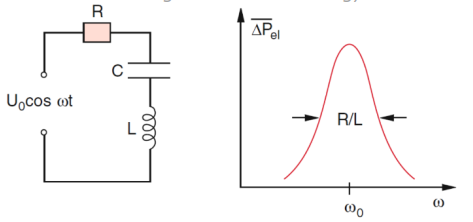
\includegraphics[width=7cm]{image/12/1.png}
\end{figure}

\paragraph{Zeichnen Sie den Schaltplan eines gedämpften Parallelschwingkreises der an eine
Wechselspannungsquelle angeschlossen ist und erstellen Sie ein Diagramm der im Schwingkreis
verbrauchten Wirkleistung als Funktion der Frequenz der Wechselspannung.}
Grenzfrequenz ist jene Frequenz, bei welcher sich die imaginären Anteile von der Spule und dem Kondensator gegenseitig aufheben. Ergo kann L und C im Schlatplan weggedacht werden.
\\
Wird L und C weggedacht, bleibt ein Kurzschluss übrig! \\
Daher Leistungsminimum bei Grenzfrequenz
\begin{figure}[H]
    \centering
    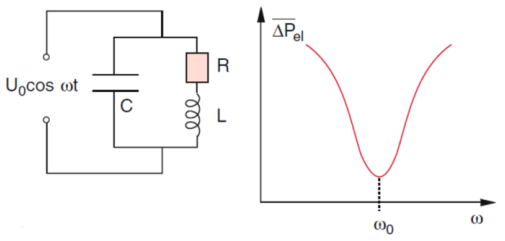
\includegraphics[width=7cm]{image/12/2.png}
\end{figure}

\paragraph{Erstellen Sie das Zeigerdiagramm für Strom und Spannung eines an eine
Wechselspannungsquelle angeschlossenen, gedämpften Serienschwingkreis für eine Frequenz unterhalb,
oberhalb und bei der Resonanzfrequenz. Zeichnen Sie auch alle Teilspannungen bzw. Ströme an den
einzelnen Bauelementen ein}.
\begin{figure}[H]
    \centering
    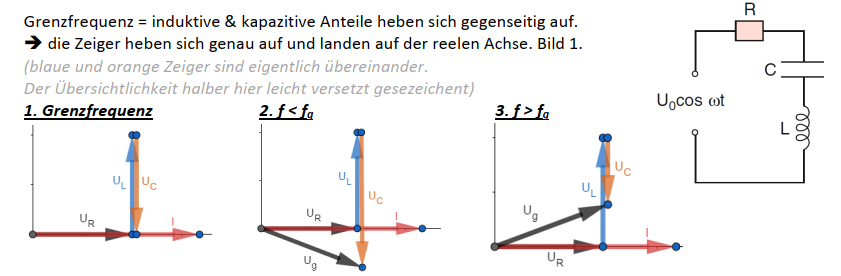
\includegraphics[width=14cm]{image/12/3.png}
\end{figure}
Bild 2:
\begin{itemize}
\item niedrige Frequenz erhöht den Widerstand am Kondensator
\item niedrige Frequenz senkt den Widerstand an der Spule
\item Hoher Widerstand an C -> hohe Spannung -> größerer Zeiger nach unten
\end{itemize}
Bild 3:
\begin{itemize}
\item hohe Frequenz erhöht den Widerstand an der Spule
\item hohe Frequenz senkt den Widerstand an der Spule
\item hoher Widerstand an C -> hohe Spannung -> größerer Zeiger nach unten
\end{itemize}

\paragraph{Gegeben sei ein gedämpfter Serienschwingkreis. Zeichnen Sie ein Diagramm des Stromes als
Funktion der Zeit nach einem Spannungssprung ($I(0)=0$; $\dot{I}(0)\neq 0$) am Schwingkreis für den
Kriechfall, den Aperiodischen Grenzfall und eine gedämpfte Schwingung}.
\begin{figure}[H]
    \centering
    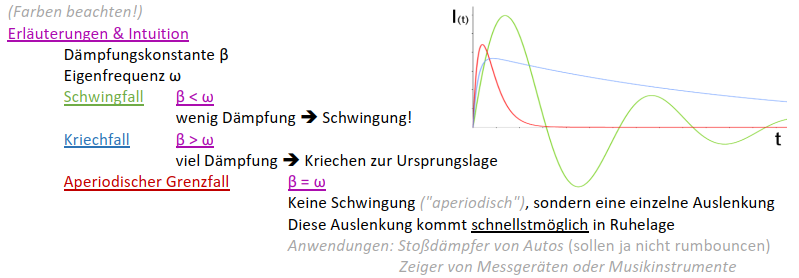
\includegraphics[width=14cm]{image/12/4.png}
\end{figure}

\paragraph{Wie sieht die Abstrahlcharakteristik (räumliche Verteilung der Leistungsabstrahlung in
großer Entfernung) eines schwingenden Dipols aus}\textbf{?}
\begin{figure}[H]
    \centering
    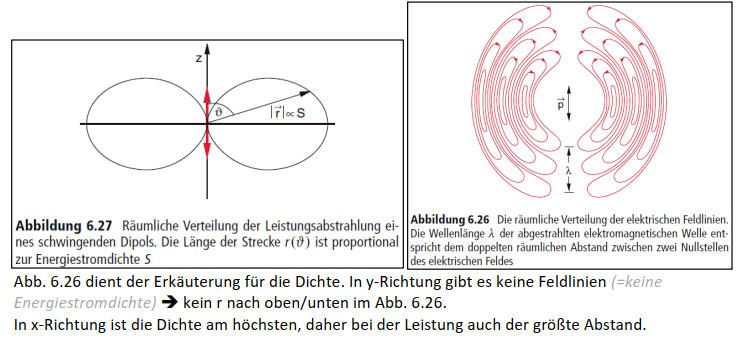
\includegraphics[width=14cm]{image/12/5.png}
\end{figure}


\paragraph{Was ist Bremsstrahlung und mit welchen Geräten wird sie technisch Erzeugt?}
Bremsstrahlung ist elektromagnetische Strahlung, die entsteht, wenn der Impuls eines geladenen Teilchens, z.B. eines Elektrons, geändert wird. Dem liegt zugrunde, dass jede Geschwindigkeitsänderung eines geladenen Teilchens mit der Absorption oder Emission von elektromagnetischer Strahlung verbunden ist (Energieerhaltung !).\\
\textbf{Technische Erzeugung:} \\
\begin{itemize}
\item Teilchenbeschleuniger
\item Röntgenröhren in der Medizin
\end{itemize}
\begin{figure}[H]
    \centering
    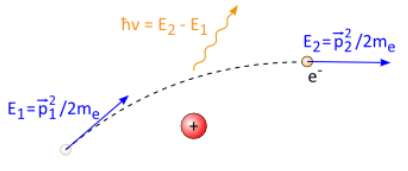
\includegraphics[width=8cm]{image/12/6.png}
\end{figure}
\textbf{Bilderläuterung:} \\
Wird z.B. ein Elektron um einen Kern gebremst, so verändert sich dessen Impuls und somit $E_{Kin}$. \\
Die Energiedifferenz wird also abgestrahlt. Dieses Phänomen nennt man Bremsstrahlung. Dieser Effekt tritt aber ebenso bei Beschleunigung auf, nicht nur bei Bremsung. Dabei wird ein Photon absorbiert (Die Energie des Photons ist dann der Betrag, mit welchem beschleunigt wird).

\newpage

\section{Elektromagnetische Wellen}

\paragraph{Was sind ebene elektromagnetische Wellen? Schreiben Sie die Gleichung für das elektrische
Feld einer ebenen, harmonischen, elektromagnetische Welle an.}

\paragraph{Skizzieren Sie zeitlichen und örtlichen Verlauf des elektrischen Feldes einer ebenen,
harmonischen, elektromagnetischen Welle. Geben Sie die Wellengleichung an und markieren Sie
Wellenlänge und Periodendauer in Ihren Skizzen. Wie gehen diese beiden Größen in die Wellengleichung
ein?}

\paragraph{Was versteht man unter linearer, elliptischer, zirkulare Polarisation bzw. unter
unpolarisiertem Licht?}

\paragraph{Skizzieren Sie den räumlichen Verlauf des elektrischen und magnetischen Feldes einer
harmonischen, ebenen elektromagnetischen Welle zu einen Zeitpunkt (Vektoren!).}

\paragraph{Was versteht man unter Energiestromdichte und Intensität? Welche Einheiten haben sie?}

\paragraph{Beschreiben Sie die Entstehung und Eigenschaften einer stehenden elektromagnetischen
Welle.}

\newpage

\section{Wellen in Materie}

\paragraph{Beschreiben Sie die Leitung elektromagnetischer Wellen zwischen zwei elektrisch
leitenden, ebenen Platten.}

\paragraph{Wellenleitung auf Kabeln: Leiten Sie einen Ausdruck für die Eingangsimpedanz
(Wellenwiderstand) eines Kabels mit bekanntem Induktivitäts- und Kapazitätsbelag her.}

\paragraph{Erklären Sie das elektromagnetische Frequenzspektrum. Welchen Spektralbereich hat UV,
sichtbares Licht, Infrarot, Mikrowellen und Radiowellen?}

\paragraph{Was versteht man unter Brechungsindex und was bedeutet ein komplexwertiger
Brechungsindex? Wie geht eine komplexwertiger Brechungsindex in die Wellengleichung ein?}

\paragraph{Schreiben Sie das Beer’sche Absorptionsgesetz an (Skizze). Erstellen Sie ein Diagramm der
Intensität als Funktion der Ausbreitungslänge der Welle.}

\paragraph{Wie sieht der frequenzabhängige Verlauf von Real- und Imaginärteil des Brechungsindex
qualitativ aus? Erstellen Sie Diagramme. Eine Absorptionslinie sollte im betrachteten
Frequenzbereich enthalten sein.}

\newpage

\section{Wellen an Grenzflächen, optische Anisotropie und Polarisation}

\paragraph{Zeichnen Sie ein Diagramm mit dem winkelabhängigen Verlauf des Reflexionsvermögens für s-
und p-polarisiertes Licht als Funktion des Einfallswinkels für Reflexion am optisch dichteren
Medium.}

\paragraph{Zeichnen Sie ein Diagramm mit dem winkelabhängigen Verlauf des Reflexionsvermögens für s-
und p-polarisiertes Licht als Funktion des Einfallswinkels für Reflexion am optisch dünneren
Medium.}

\paragraph{Was bedeutet „Reflexionskoeffizient“ und „Reflexionsvermögen“ (Reflektivität),
„Transmissionskoeffizient“ und „Transmissionsvermögen“ (Transmissionsgrad)? Wie groß ist das
Reflexionsvermögen einer Grenzfläche zwischen zwei transparenten Medien bei Lichteinfall senkrecht
auf die Grenzfläche.}

\paragraph{Erklären Sie mithilfe einer Skizze die Begriffe „Einfallswinkel“, „Reflexionswinkel“, „Brechungswinkel“, „Einfallsebene“. Was bedeutet s- bzw. p-Polarisation? Leiten Sie das Reflexions-
und Brechungsgesetz her.}

\paragraph{Was ist der Brewsterwinkel? Erstellen Sie eine Skizze einer Luft-Glas Grenzfläche und
zeichnen Sie alle mögliche Brewsterwinkel ein. Wie ist der Polarisationszustand der reflektierten
und transmittierten Welle bei unpolarisierter einfallender Welle?}

\paragraph{Was ist Totalreflextion und unter welchen Bedingungen tritt sie auf? Welche Rolle spielt
die Polarisation dabei?}

\paragraph{Was sind optisch anisotrope Kristalle und wie lassen sich die unterschiedlichen
Richtungen der elektrischen Feldstärke und der dielektrischen Verschiebungsdichte mit dem
mechanischen Analogmodell verstehen? Wie sieht der Zusammenhang zwischen elektrischer Feldstärke und dielektrischer Verschiebungsdichte dabei formal aus?}

\paragraph{Was sind optisch einachsige bzw. optisch zweiachsige Kristalle. Wodurch unterscheidet
sich deren $\epsilon$-Tensoren in Hauptachsendarstellung? Was ist die optische Achse eines
doppelbrechenden Kristalles?}

\paragraph{Zeichnen und erklären Sie eine zweidimensionale Darstellung des Indexellipsoides eines
optisch einachsigen Kristalles. Wie unterscheidet sich das Verhalten von ordentlichem und
außerordentlichem Strahl bei optisch einachsigen Kristallen?}

\paragraph{Beschreiben Sie die Funktion eines dichroitischen und eines Glan-Thompson Polarisators.
(Skizze!)}

\paragraph{Beschreiben Sie die Funktion eines $\lambda/4$-Plättchens. Welche Bedingungen muss es
erfüllen? (Skizze!)}

\paragraph{Beschreiben Sie die Funktion eines $\lambda/2$-Plättchens. Welche Bedingungen muss es
erfüllen? (Skizze!)}

\paragraph{Was ist optische Aktivität und wie lässt sich eine Platte aus optisch aktivem Material
von einer $\lambda/2$-Platte unterscheiden?}

\newpage

\section{Geometrische Optik I}

\paragraph{Nennen Sie die Axiome der Geometrischen Optik und erklären Sie unter welchen Bedingungen
diese gut erfüllt sind.}

\paragraph{Beschreiben Sie die Abbildung in einem ebenen Spiegel. Zeichen Sie den Strahlengang für
die Abbildung von zwei Gegenständen in unterschiedlichem Abstand vom Spiegel.}

\paragraph{Erklären Sie den Unterschied zwischen einem reellen und einem virtuellen Bild.}

\paragraph{Zeichnen Sie die 3 Konstruktionsstrahlen bei der Abbildung durch eine dünne Linse.
Erklären sie, warum diese Strahlen für die Bildkonstruktion gewählt werden und warum sie so
verlaufen wie sie es eingezeichnet haben. Zeichen Sie Bildweite, Gegenstandsweite und Brennweite
ein.}

\paragraph{Konstruieren Sie das Bild eines Gegenstandes durch eine dünne Sammellinse wenn (a) der
Gegenstand mehr als $2f$ von der Linse entfernt ist und (b) wenn der Gegenstand weniger als $2f$ von
der Linse entfernt ist. Dabei ist $f$ die Brennweite der Linse.}

\paragraph{Konstruieren Sie das Bild eines Gegenstandes durch eine dünne Zerstruungslinse wenn (a)
der Gegenstand mehr als $2f$ von der Linse entfernt ist und (b) wenn der Gegenstand weniger
als $2f$ von der Linse entfernt ist. Dabei ist $f$ die Brennweite der Linse.}

\paragraph{Wie ist die Vergrößerung definiert? Zeichen Sie die Abbildung mit einer dünnen
Sammellinse und leiten Sie eine Formel zur Berechnung der Vergrößerung aus Bild- und
Gegenstandsweite her.}

\paragraph{Wie ist die Vergrößerung definiert? Zeichen Sie die Abbildung mit einer dünnen
Zerstreuungslinse und leiten Sie eine Formel zur Berechnung der Vergrößerung aus Bild- und
Gegenstandsweite her.}

\newpage

\section{Geometrische Optik II}

\paragraph{Erklären Sie die Bedeutung der Hauptebenen dicker Linsen sowie die Bildkonstruktion bei
dicken Linsen.}

\paragraph{Zeichen Sie zwei Sammellinsen, deren Abstand kleiner als die kleinere von den beiden
Brennweiten ist. Konstruieren Sie den Strahlengang für die Abbildung eines Objektes durch
das Linsensystem.}

\paragraph{Zeichen Sie zwei Sammellinsen, deren Abstand größer als die Summe der beiden
Brennweiten ist. Konstruieren Sie den Strahlengang für die Abbildung eines Objektes durch
das Linsensystem.}

\paragraph{Nennen und erklären Sie die unterschiedlichen Abbildungsfehler, die bei einer Abbildung
mit einer Linse entstehen können.}

\newpage
% Start Elias 
\section{Interferenz}

\myparagraph{Was versteht man unter „Interferenz“ und „Kohärenz“?}

\textbf{Interferenz} ist die Überlagerung von Teilwellen. Die Folgen von konstruktiver und destruktiver Interferenz werden als Interferenzmuster bezeichnet.\\
\textbf{Kohärenz} Wellen nennt man hkhärent, wenn sie die gleiche Phasenbeziehung beibehalten. Dabei unterscheidet man:
\begin{itemize}
    \item \textbf{räumliche Kohärenz: } die Phasendifferenz zwischen Teilwellen bleibt räumlich konstant
    \item \textbf{zeitliche Kohärenz: } die Phasendifferenz zwischen Teilwellen bleibt zeitlich konstant
\end{itemize}

\myparagraph{Erklären Sie die Beugung von Licht am Young‘schen Doppelspalt durch Interfernz. Bei
Welchen Winkeln trete im Fraunhoferschen Limit Intensitätsmaxima auf? Leiten Sie die
Formel für diese Winkel her.}

Einfallende Wellen treffen auf die beiden Spalten $S_1$ und $S_2$ und werden jeweils gebeugt. Am Schirm (B) bildet sich so ein Interferenzmuster. 
Dieses Interferenzmuster lässt sich durch die unterschiedliche Weglänge, welche von den Teilstrahlen zurückgelegt wird erklären.
\begin{figure}[H]
    \centering
    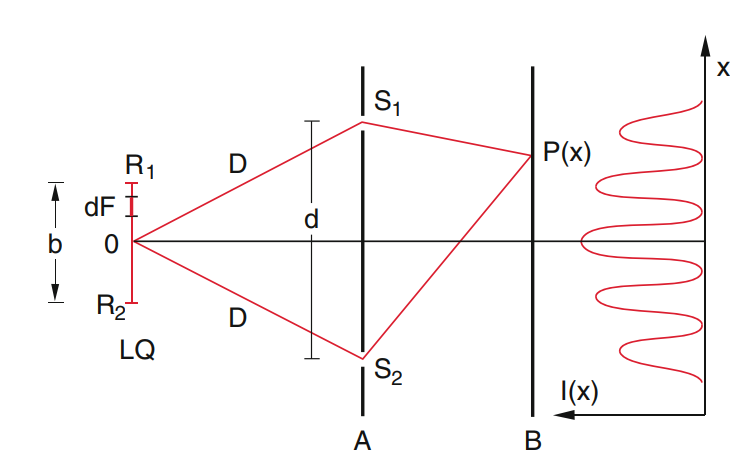
\includegraphics[width=8cm]{image/18_Interferenz/Youngscher Doppelspalt.png}
\end{figure}
Frauenhofer Limit $\rightarrow$ großer Abstand zwischen Quelle und Schirm, bzw. kleine Quelle.
\begin{figure}[H]
    \centering
    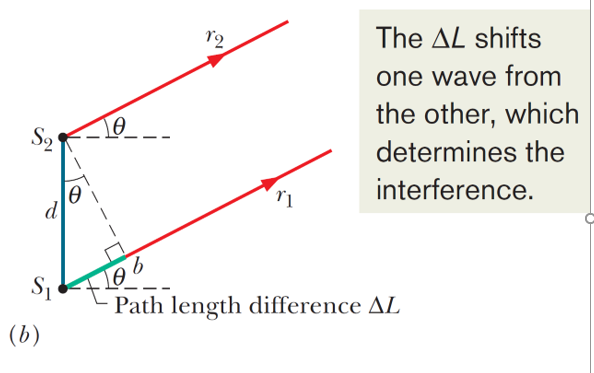
\includegraphics[width=8cm]{image/18_Interferenz/Doppelspalt_Wegunterschied.png}
\end{figure}
Der Winkel $\theta$ beschreibt die Verbindung eines beliebigen Punktes P mit der Mitte der beiden Spalte. 
In Abb. b) sieht man, dass $\Delta$ L (grün) die Phasendifferenz der beiden Strahlen r1 und r2 bestimmt. Beide 
Strahlen sind annähernd parallel dank großem Abstand zwischen Schirm und Doppelspalt. 
\[\sin \theta = \frac{\Delta L}{d} \hspace{1cm} \rightarrow \hspace{1cm} \Delta L = d \cdot \sin \theta\]
Ist $\Delta$ L ein Vielfaches n$\in\mathbb{N}$ der Wellenlänge $\lambda$, entsteht konstruktive Interferenz/ein Maximum.
\[d \cdot \sin \theta = n \cdot \lambda\]
Somit ergeben sich die die Intensitätsmaxima unter folgendem Winkel:
\begin{equation}
    \label{eq:Intensitaetsmaxima_Young_Doppelspalt}
    \arcsin \theta = \frac{n \cdot \lambda}{d}
\end{equation}


\paragraph{Beschreiben Sie den Aufbau und Funktion eines Michelson-Interferometers und schreiben
sie einen Ausdruck für die Intensität am Detektor als Funktion der Längendifferenz der
Lichtwege an.}

\paragraph{Was versteht man unter „zeitlicher Kohärenz“? Wovon hängt sie ab bzw. wie kann man sie
beeinflussen? Mit welchem Gerät könnte man sie wie bestimmen?}

\paragraph{Was versteht man unter „räumlicher Kohärenz“? Wovon hängt sie ab bzw. wie kann man sie
beeinflussen? Mit welchem Gerät könnte man sie wie bestimmen?}

\paragraph{Zeichnen Sie den prinzipiellen Aufbau / Strahlengang eines Sagnac und eines Mach-Zehnder Interferometers.}

\paragraph{Erklären Sie Aufbau, Funktion und Transmissionsverhalten eines
Fabry-Perot-Interferometers. Skizzieren Sie den spektralen Verlauf der Transmission als Funktion der
Finesse. Wie ist die Finesse definiert?}

\paragraph{Beschreiben Sie die Funktionsweise einer einfachen Antireflexbeschichtung aus einer
dielektrischen Schicht.}

\newpage

\section{Beugung}

\paragraph{Leiten Sie die Formel für die Intensitätsverteilung einer regelmäßigen Anordnung von
kohärenten Emittern her und skizzieren Sie diese in einem Diagramm (Intensität vs.
Winkel).}

\paragraph{Beugung am Einzelspalt: Schreiben Sie einen Ausdruck für die Intensitätsverteilung im
Fraunhofer‘schen Beugungsbild eines einzelnen, mit einer ebenen Welle beleuchteten
Spaltes an und skizzieren Sie diese in einem Diagramm. Bei welchem Winkel liegt das erste
Beugungsminimum und wie lässt sich dies einfach erklären?}

\paragraph{Beugung am Gitter: Schreiben Sie einen Ausdruck für die Intensitätsverteilung im
Fraunhofer‘schen Beugungsbild eines mit einer ebenen Welle beleuchteten Spaltgitters an
und skizzieren Sie diese in einem Diagramm. Bei welchen Winkeln liegen die Hauptmaxima
und wie lassen sich diese Winkel einfach erklären?}

\paragraph{Skizzieren Sie den Aufbau eins geblazeten Gitters und erklären Sie dessen Funktion.}

\paragraph{Erklären und Skizzieren Sie Aufbau und Funktion einer Fresnel‘schen Zonenplatte.}

\paragraph{Beugung am Gitter: Schreiben Sie einen Ausdruck für die Intensitätsverteilung im
Fraunhofer‘schen Beugungsbild einer mit einer ebenen Welle beleuchteten Kreisblende an
und skizzieren Sie diese in einem Diagramm.}

\newpage

\section{Optische Instrumente I}

\paragraph{Skizzieren und beschreiben Sie den Aufbau des Auges. Welche Arten von Sehzellen sind
vorhanden und welche spektrale empfindlichkeit haben diese (Diagramm)?}

\paragraph{Zeichnen Sie den Strahlengang für eine Lupe, wobei das Auge auf unendlich eingestellt
sein soll um ein scharfes Bild des Gegenstandes durch die Lupe zu sehen. Leiten Sie einen Ausdruck
für die Winkelvergrößerung der Lupe her.}

\paragraph{Zeichnen Sie den prinzipiellen Aufbau eines Mikroskopes mit dem Abbildungsstrahlengang
(von einem Objektpunkt zum Bildpunkt). Wie ist die Vergrößerung definiert und wie kann man sie
berechnen?}

\paragraph{Zeichnen Sie den prinzipiellen Aufbau eines Keplerschen Fernrohres mit dem
Abbildungsstrahlengang (von einem weit entfernten Objektpunkt zum Bildpunkt). Wie ist die
Vergrößerung definiert und wie kann man sie berechnen?}

\paragraph{Zeichnen Sie den prinzipiellen Aufbau eines Gallileischen Fernrohres mit dem
Abbildungsstrahlengang (von einem weit entfernten Objektpunkt zum Bildpunkt). Wie ist die
Vergrößerung definiert und wie kann man sie berechnen?}

\paragraph{Zeichnen Sie den prinzipiellen Aufbau eines Projektors mit dem Abbildungsstrahlengang
und dem Beleuchtungsstrahlengang.}

\paragraph{Was versteht man unter Schärfentiefe und Lichtstärke? Wie kann man diese Größen bei
einer gegebenen Linse beeinflussen? Beschreiben Sie wie sich die Größen ändern.}

\paragraph{Welchen Einfluß hat Beugung auf die Abbildung mit einer Linse? Wie ist das
Auflösungsvermögen definiert? Wie groß ist das Auflösungsvermögen einer Linse mit gegebenem
Durchmesser und Brennweite für die Abbildung weit entfernter Gegenstände?}

\newpage

\section{Optische Instrumente II}

\paragraph{Erklären Sie kurz die Abb‘esche Abbildungstheorie zur Bildenstehung}

\paragraph{Berechnen Sie am Beispiel eines Liniengitters das Auflösungsvermögen einer Abbildung
durch ein Objektiv.}

\paragraph{Was besagt die Abbe‘sche Sinusbedingung? Erklären Sie anhand eines Gitters als Objekt
warum sie gelten muss, um eine gute Abbildung zu erreichen.}

\paragraph{Zeichnen Sie den Strahlengang für die Abbildung eines Gitters durch eine oder zwei Linsen
sowohl für das Beugungsbild (und weiterer Strahlengang) als auch für das Bild. Achten Sie
auf die korrekte Konstruktion der Bild- bzw. Beugungsbildpunkte.}

\paragraph{Schreiben Sie das Auflösungsvermögen für ein Mikroskopobjektiv an, wenn die
Gegenstandspunkte inkohärent leuchten bzw. inkkohärent beleuchtet sind. Wie ist die Numerische
Apertur definiert (Skizze)?}

\paragraph{Zeichen Sie den optischen Strahlengang eines Gittermonochromators (Czerny-Turner) und
bezeichnen Sie alle wesentlichen Elemente.}

\paragraph{Wie ist das spektrale Auflösungsvermögen definiert? Schreiben Sie einen Ausdruck für das
spektrale Auflösungsvermögen eins Gittermonochromators an.}

\end{document}
